\documentclass[12pt]{article}

\usepackage{lmodern}
\usepackage[T1]{fontenc}
\usepackage[utf8]{inputenc}
\usepackage[spanish, activeacute]{babel}
\usepackage{listings}
\usepackage{enumitem}
\usepackage{graphicx}
\usepackage{float}
\usepackage[hidelinks]{hyperref}

\graphicspath{ {assets/images/} }

\title{Practica 01 - Instalación de Herramientas }

\author{ 
    Wilson Aguilar \\
    \textsc{Plataformas Web} 
}

\begin{document}

\maketitle

\begin{abstract}
    En el presente documento se detalla la configuración del entorno de trabajo para la materia de Plataformas Web, donde veremos las herramientas principales que vamos a utilizar. El sistema utilizado es ElementyOs 5.1.2, una distribución de linux basada en Ubuntu 18.04LTS.
\end{abstract}

\section{Instalación de Visual Studio Code}

Para la Instalación de VsCode optamos por agregar el repositorio del programa al sistema para tener acceso a las actualizaciones de una manera mas rápida.
Para ello abrimos la terminal y ejecutamos los siguientes comandos.

\begin{lstlisting}[language=bash]
$ curl https://packages.microsoft.com/keys/microsoft
.asc | gpg --dearmor > packages.microsoft.gpg

$ sudo install -o root -g root -m 644 packages
.microsoft.gpg /usr/share/keyrings/

$ sudo sh -c 'echo "deb [arch=amd64 
signed-by=/usr/share/keyrings/packages.microsoft.gpg] 
https://packages.microsoft.com/repos/vscode 
stable main" > /etc/apt/sources.list.d/vscode.list'

\end{lstlisting}

Después de esto ya tendremos agregado el repositorio de vscode en nuestro sistema. Ahora actualizamos los repositorios del sistema e instalamos de forma normal los paquetes \lstinline{apt-transport-https} y \lstinline{code} para una Instalación segura.

\subsection{Extensiones}
Para mejorar el proceso de desarrollo en VsCode instalaremos algunas extensiones que nos ayudarán a realizar tareas de manera mas sencilla.

\begin{description}
    \item[HTML CSS Support 0.2.3]
          Agrega el soporte de CSS para archivos\\
          HTML.
    \item[JavaScript (ES6) code snippets] Agrega snippets de JavaScript y TypeScript.
    \item[JS-CSS-HTML Formatter] Ayuda a formatear el código. Soporta JS,\\ HTML, CSS y Json.
    \item[Terminal] Permite ejecutar una terminal del sistema desde el mismo editor.
    \item[TypeScript Importer] Importa automaticamente librerias que estemos \\usando.
\end{description}

\begin{figure}[H]
    \centering
    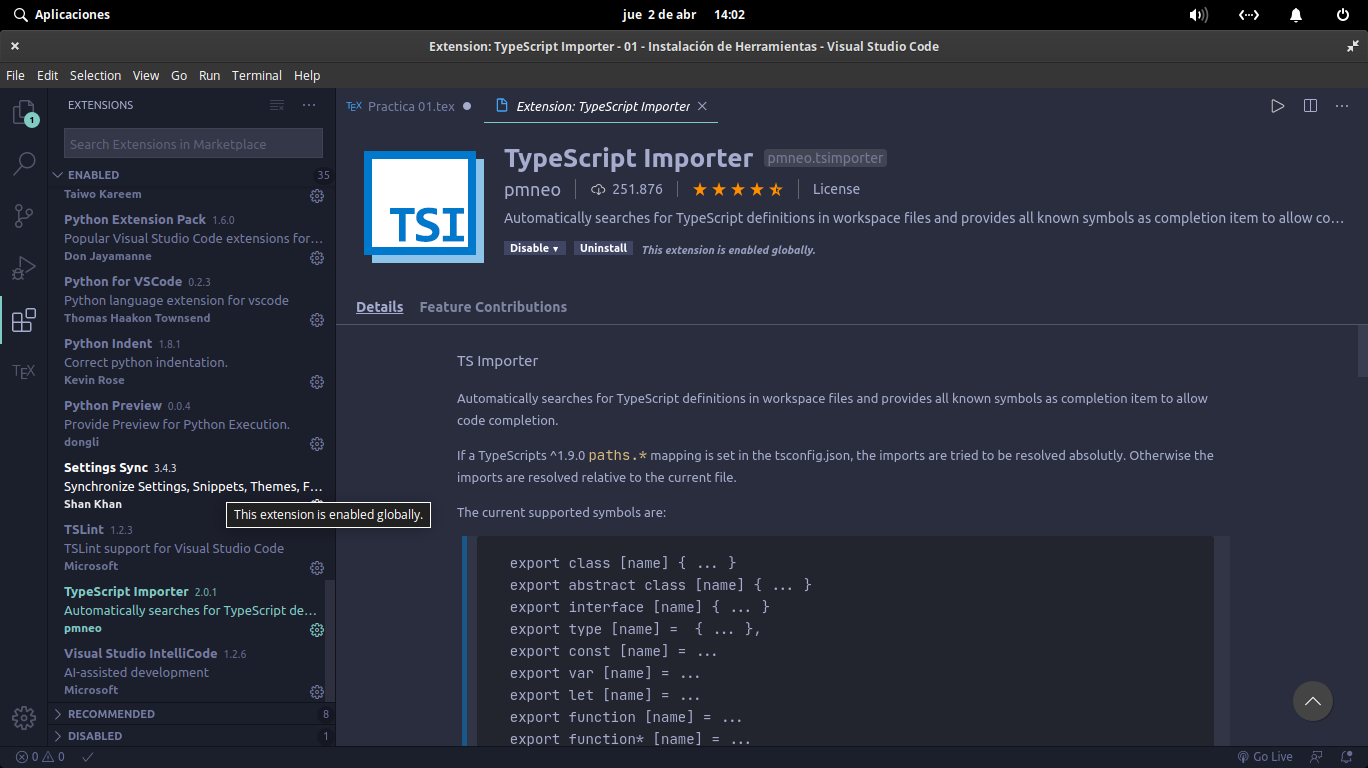
\includegraphics[scale=0.28]{vscode.png}
    \caption{Interfaz de VsCode con algunas extesiones instaladas}
\end{figure}

\section{Intalaición Git}
Para instalar Git abrimos una terminal del sistema e ingresamos el comando:

\begin{lstlisting}[language=bash]
$ sudo apt install git
\end{lstlisting}

Después configuramos nuestro git con nuestras credenciales de GitHub.

\begin{lstlisting}
$ git config --global user.name "Wilson Aguilar"
$ git config --global user.email "waguilars@est.ups.edu.ec"
\end{lstlisting}

\begin{figure}[H]
    \centering
    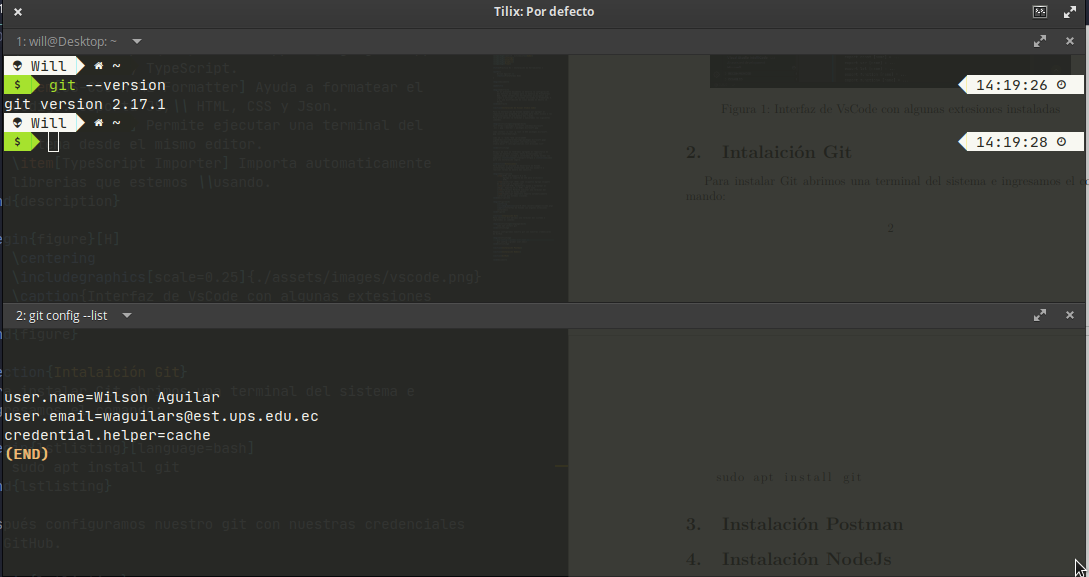
\includegraphics[scale=0.35]{git.png}
    \caption{Git instalado y configurado.}
\end{figure}

\section{Instalación Postman}
Para postman instalaremos un gestor de paquetes que contiene postman ya que el gestor por defecto que tenemos no lo trae y no hay repositorio para agregar.

Instalaremos snapd desde apt.

\begin{lstlisting}
    $ sudo apt install snapd
\end{lstlisting}

Una vez instalado snap procedemos a instalarlo con este gestor.

\begin{lstlisting}
    $ sudo snap install postman
\end{lstlisting}

\begin{figure}
    \centering
    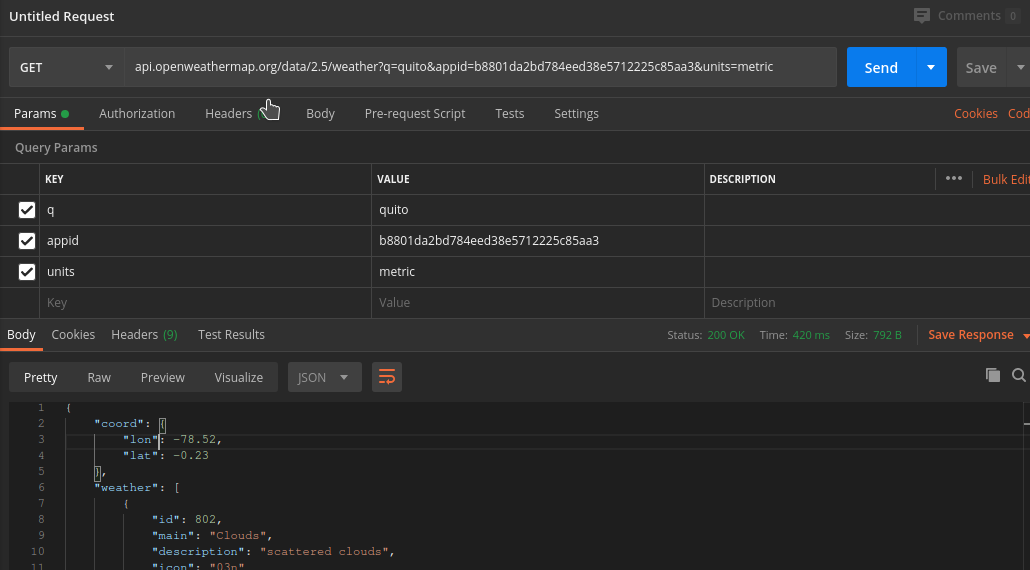
\includegraphics[scale=0.28]{postman.png}
    \caption{Postman instalado.}
\end{figure}

\section{Instalación NodeJs}
En el caso de node haremos algo similar a lo que hicimos para vscode, agregaremos el repositorio y luego instalaremos nodejs.

En una terminal ejecutamos lo siguiente:

\begin{lstlisting}[language=bash]
# En caso querer la version 13
$ curl -sL https://deb.nodesource.com/setup_13.x | 
sudo -E bash -

$ sudo apt-get install -y nodejs

# En caso de querer la version 12
$ curl -sL https://deb.nodesource.com/setup_12.x | 
sudo -E bash -

$ sudo apt-get install -y nodejs

\end{lstlisting}

\begin{figure}[H]
    \centering
    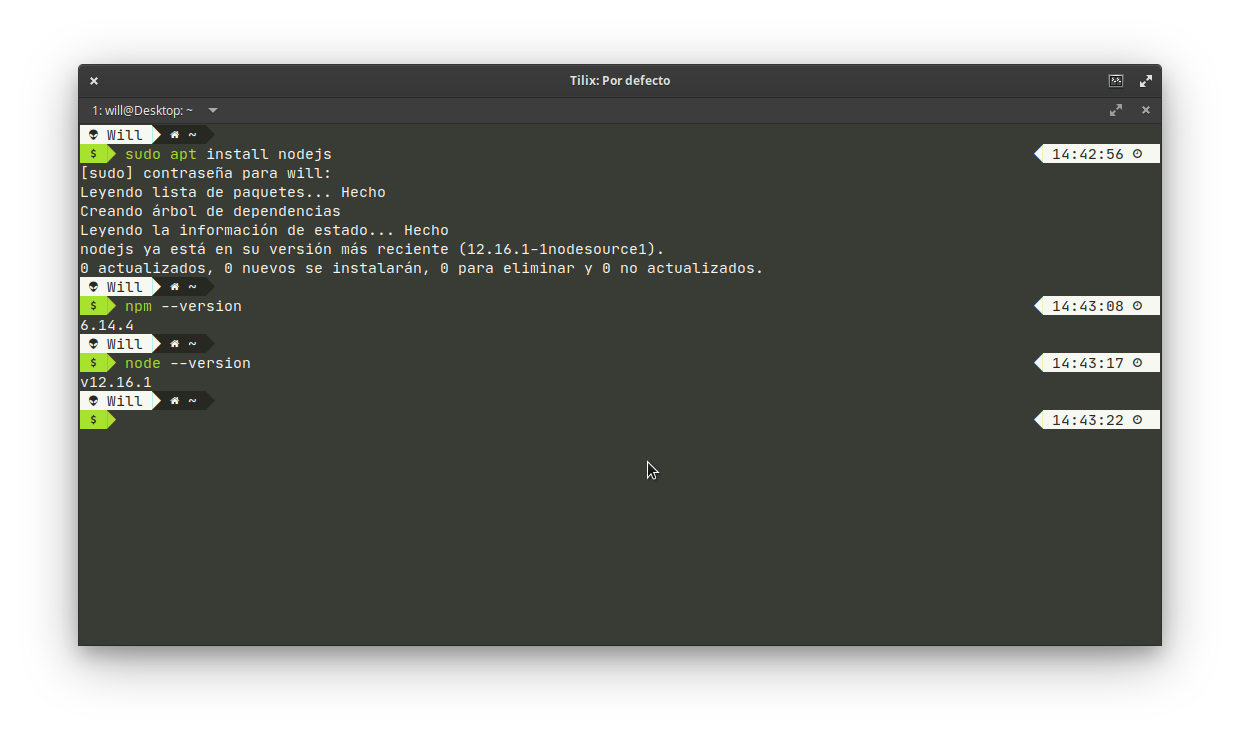
\includegraphics[scale=.3]{node.png}
    \caption{NodeJs instalado en el sistema.}
\end{figure}


\section{GitHub}

Por último actualizamos nuestro perfil de GitHub.

\begin{figure}[H]
    \centering
    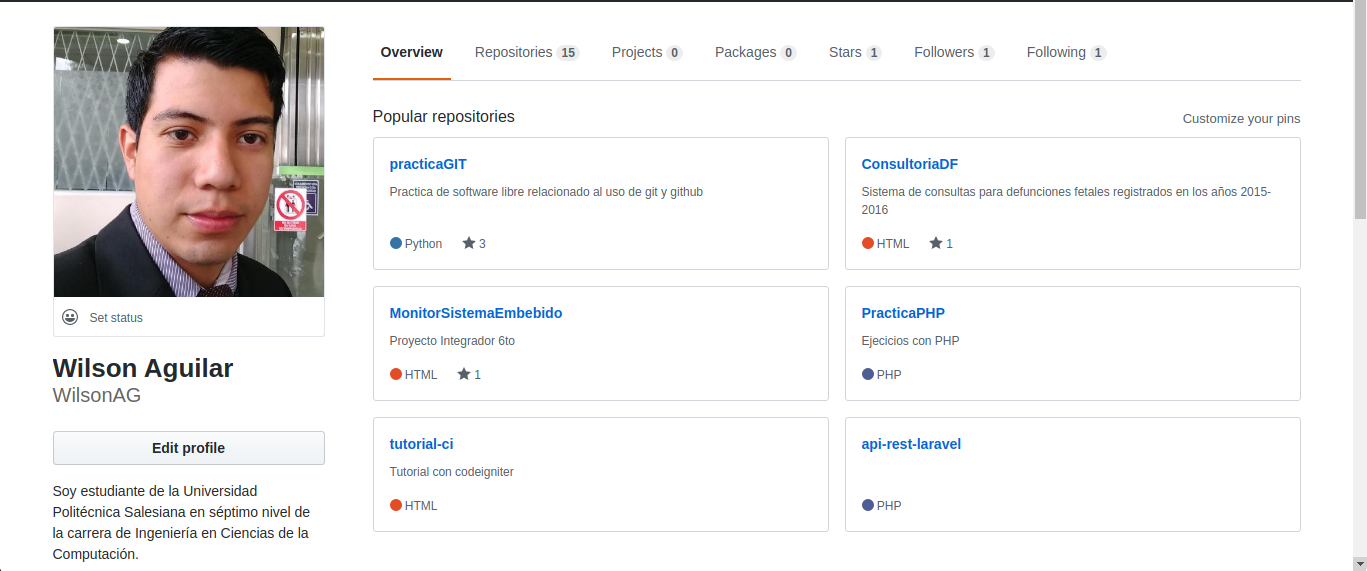
\includegraphics[scale=0.28]{github.png}
    \caption{Perfil de GitHub.}
\end{figure}

Perfil de GitHub: \url{https://github.com/WilsonAG}

\end{document}
